\documentclass[11pt]{report}
\usepackage{amsmath}
\usepackage{amssymb}
\usepackage{amsfonts}
\usepackage{mathtools}
\usepackage{amsthm}
\usepackage{ragged2e}
\usepackage[hidelinks]{hyperref}
\usepackage{float}
\usepackage{pgf,tikz}
\usepackage[shortlabels]{enumitem}
\usepackage{color}
\usepackage{pgfplots}
\usepackage[margin = 1 in]{geometry}
\usepackage{mathrsfs}
\usetikzlibrary{arrows}
\usepackage{multicol}
\usepackage{fancyhdr}
\pagestyle{fancy}
\usepackage{multirow}
\usepackage{graphicx}
\usepackage{psfrag}
\usepackage{listings}
\renewcommand{\footrulewidth}{0.4pt}

\newtheorem{theorem}{Theorem}[chapter]
\newtheorem{defn}{Definition}[chapter]
\newtheorem{lemma}{Lemma}[chapter]

\theoremstyle{definition}
\newtheorem{proposition}{Proposition}[chapter]
\newtheorem{remark}{Remark}[chapter]
\newtheorem{example}{Example}[chapter]

\newcommand{\user}{}
\newcommand{\xlr}[2]{#1 \left(#2\right)}
\newcommand{\clr}[2]{#1 \left\{ #2 \right\}}
\newcommand{\rank}{\mathrm{rank}}
\lhead{ECE 530 - Fall 2023 at University of Illinois at Urbana-Champaign}
\rhead{HW1}
\lfoot{Author: \textcolor{red}{Eric Silk, esilk2}}
\rfoot{Due: Wednesday, Sep 6}
\begin{document}


\section*{Problem 1: Newton Raphson}
\subsection*{Problem Statement}
\subsubsection*{a}
Using Newton-Raphson, solve the following system of equations in $\mathbb{R}^2$:
\[ f_1(x) \coloneqq 4x_2^2+4x_2+52x_1-19 = 0 \]
\[ f_2(x) \coloneqq 169x_1^2 + 3x_2^2 + 111x_1 - 10x_2 - 10 = 0 \]
starting from $x^0 = (5, 0)$.

Report $x^1$ and $x^2$. Terminate your iteration when the 2-norm of $f$ is less
than $10^{-10}$.  Report if it does not converge in 100 iterations. If it
converges, report $x^*$ and the iteration count.

Plot the error magnitudes $\|x^k-x^*\|$ as a function of $k$ on a semilog plot.

\subsubsection*{b}
Repeat (a), but with forward-difference approximation, using $h=0.5$.

\subsubsection*{b}
Repeat (a), but with center-difference approximation, using $h=0.5$.

\subsubsection*{d}
Repeat (a), but using Jacobian surrogates defined by Broyden's method. Clearly
state how you start the sequence of Jacobian surrogates and how you choose
$x^1$.

\subsubsection*{e}
Vary the starting point appropriately and discuss qualitatively how the
iterative process in parts a-d behave. If you have to choose between methods
b-d, which one would you choose? Will this change if evaluation of $f$ is much
more computationally expensive?

\subsection*{Solution}
\subsubsection*{a-e}
See code at end of document for implementation, or my repo here:
\begin{center}
	\href{https://github.com/eric-silk/ECE530}{https://github.com/eric-silk/ECE530}
\end{center}

Values requested ($x^1$, $x^2$, iteration count) are reported in the subplot
titles.  Specific to part (e), in general it appears that the symbolic and
center difference approximation methods tend to behave \textit{very} similarly,
and typically converge in far fewer iterations than the forward-difference or
Broyden's method; however, these methods also appear to fail in cases where the
forward-difference and Broyden's method do not. This may simply be an artifact
of the relatively low limit on iterations, but it is worth noting.

From this, for an arbitrary function, I'd probably pick Broyden's method (or
some other quasi-Newton method), especially as the computational cost of each
function evaluation increases.  It requires only one evaluation of $f$ per
iterate (which can quickly become the most significant cost), and empirically
demonstrates good convergence properties in this limited set of experiments.

\begin{figure}
	\centering
	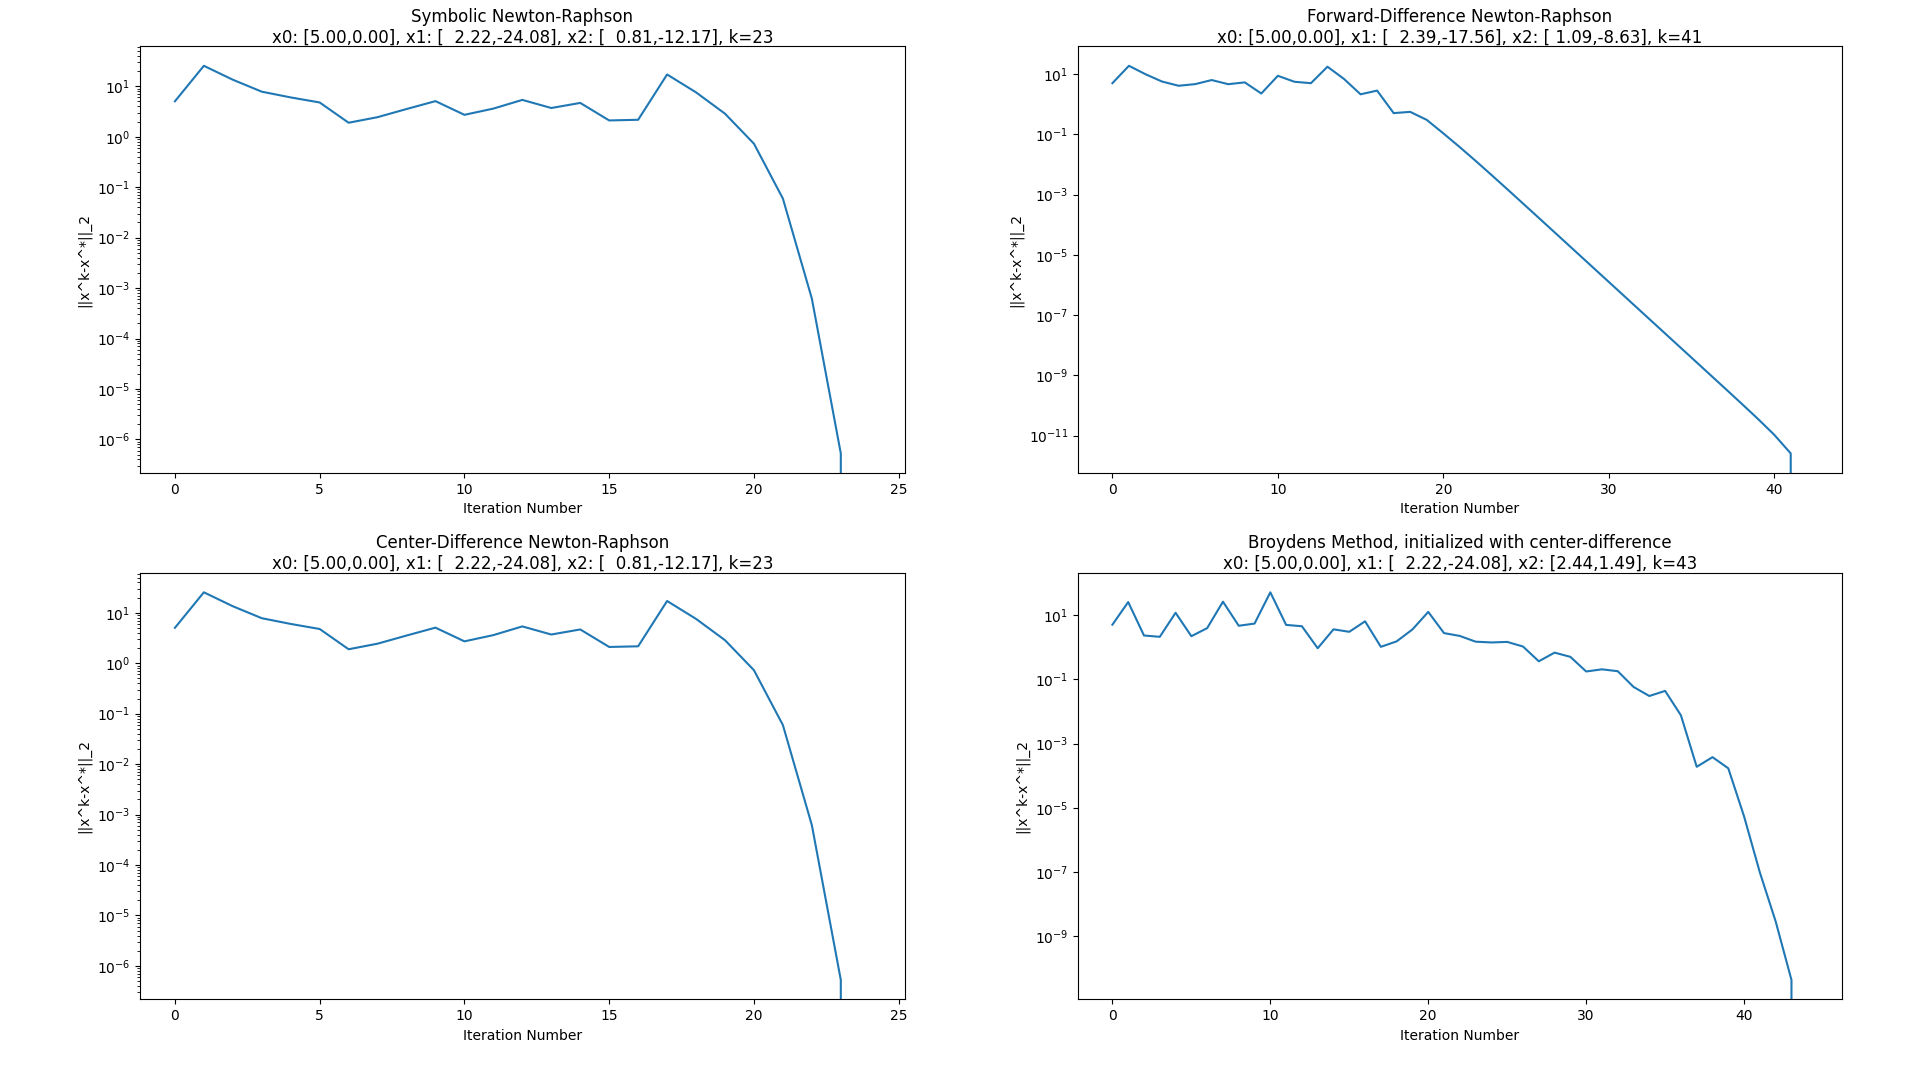
\includegraphics[width=1.25\textwidth, angle=90]{Figure_1.png}
	\caption{The four methods, started from $(5, 0)$}
\end{figure}
\begin{figure}
	\centering
	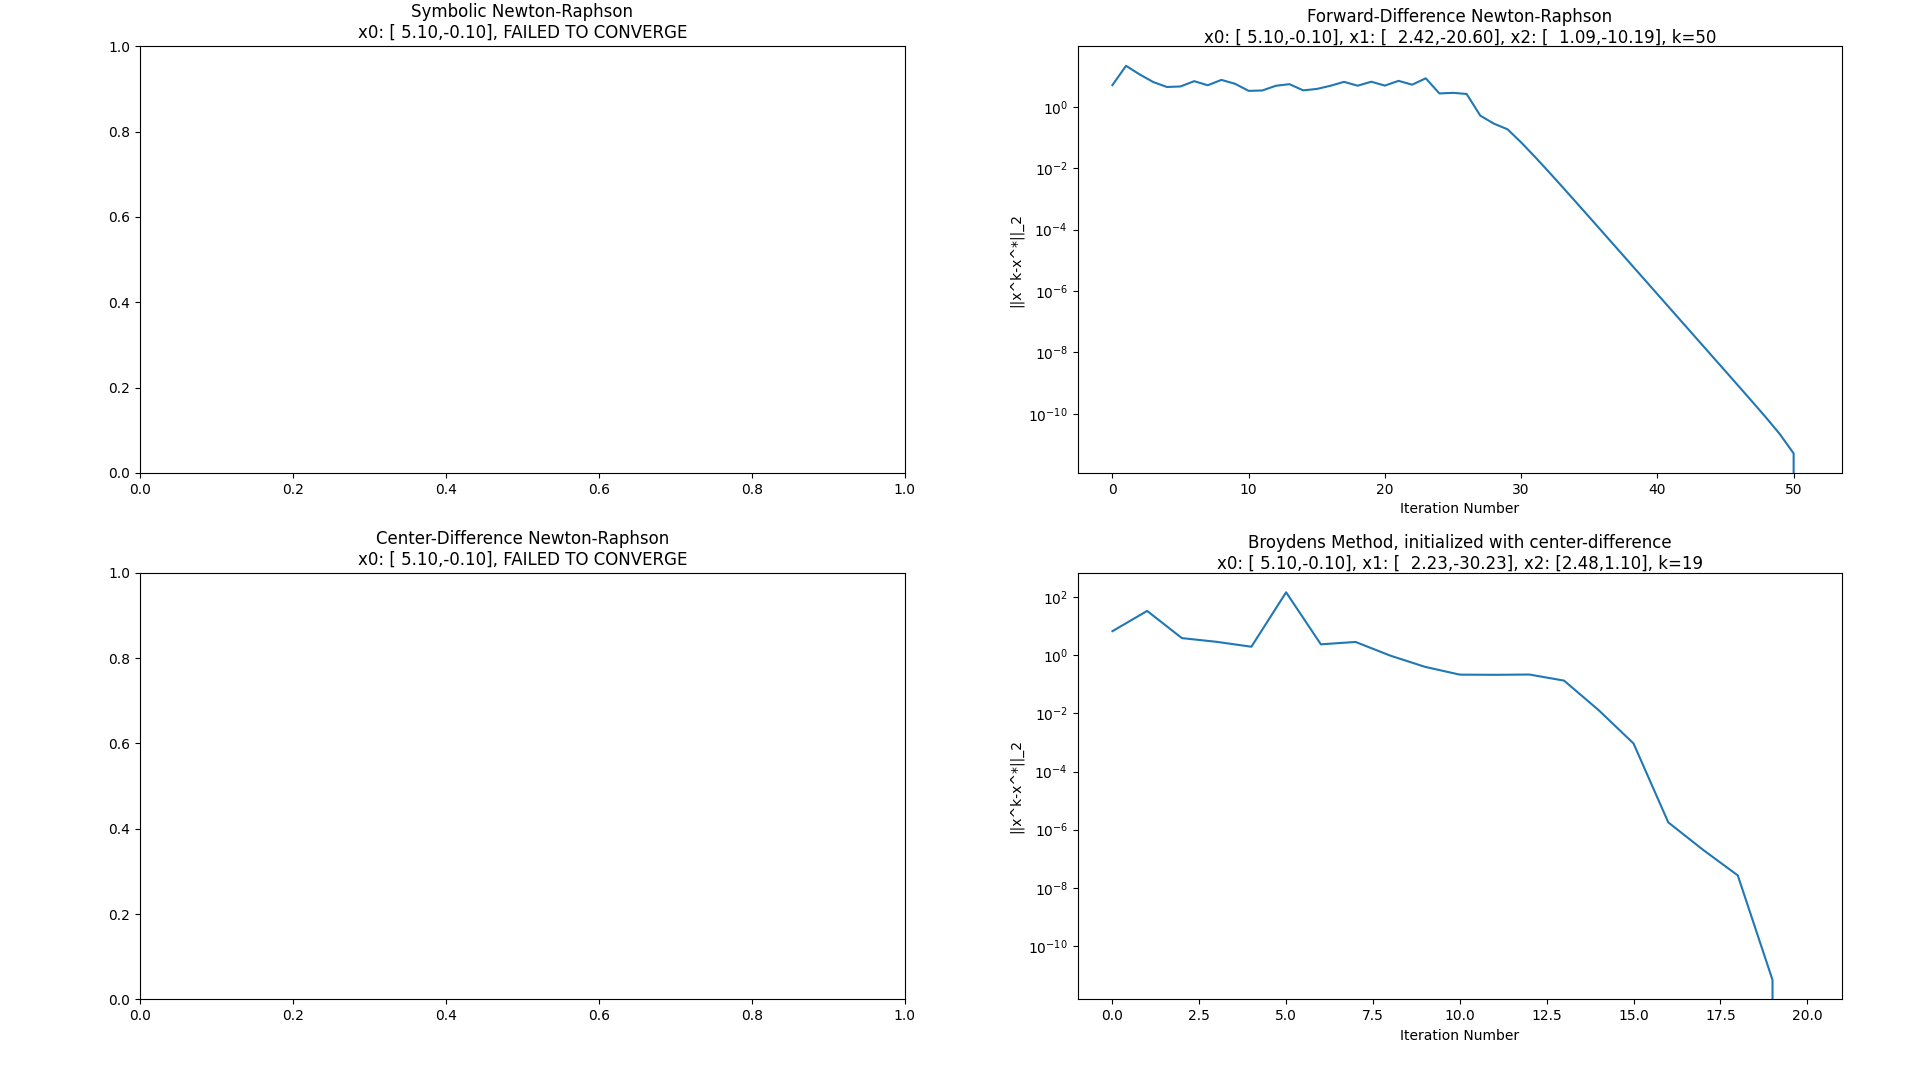
\includegraphics[width=1.25\textwidth, angle=90]{Figure_2.png}
	\caption{The four methods, started from $(5.1, -0.1)$}
\end{figure}
\begin{figure}
	\centering
	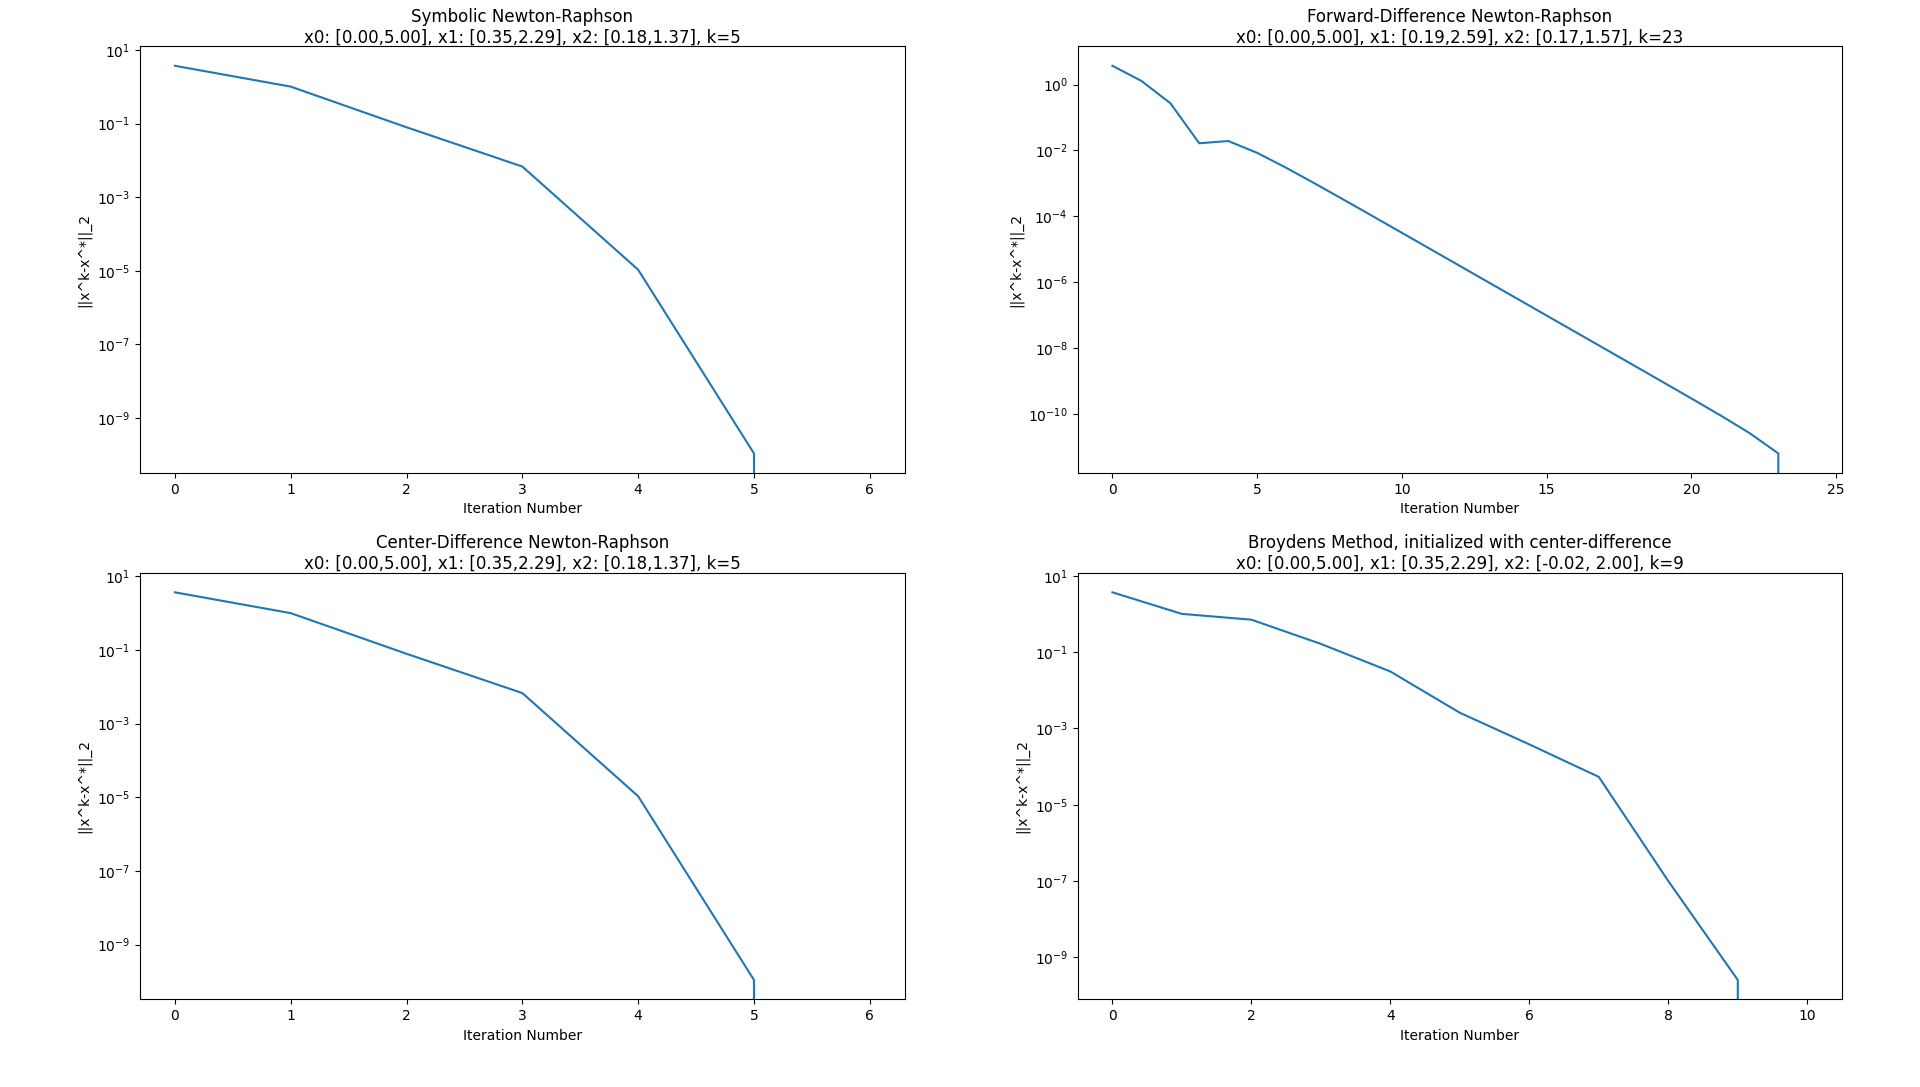
\includegraphics[width=1.25\textwidth, angle=90]{Figure_3.png}
	\caption{The four methods, started from $(0, 5)$}
\end{figure}
\begin{figure}
	\centering
	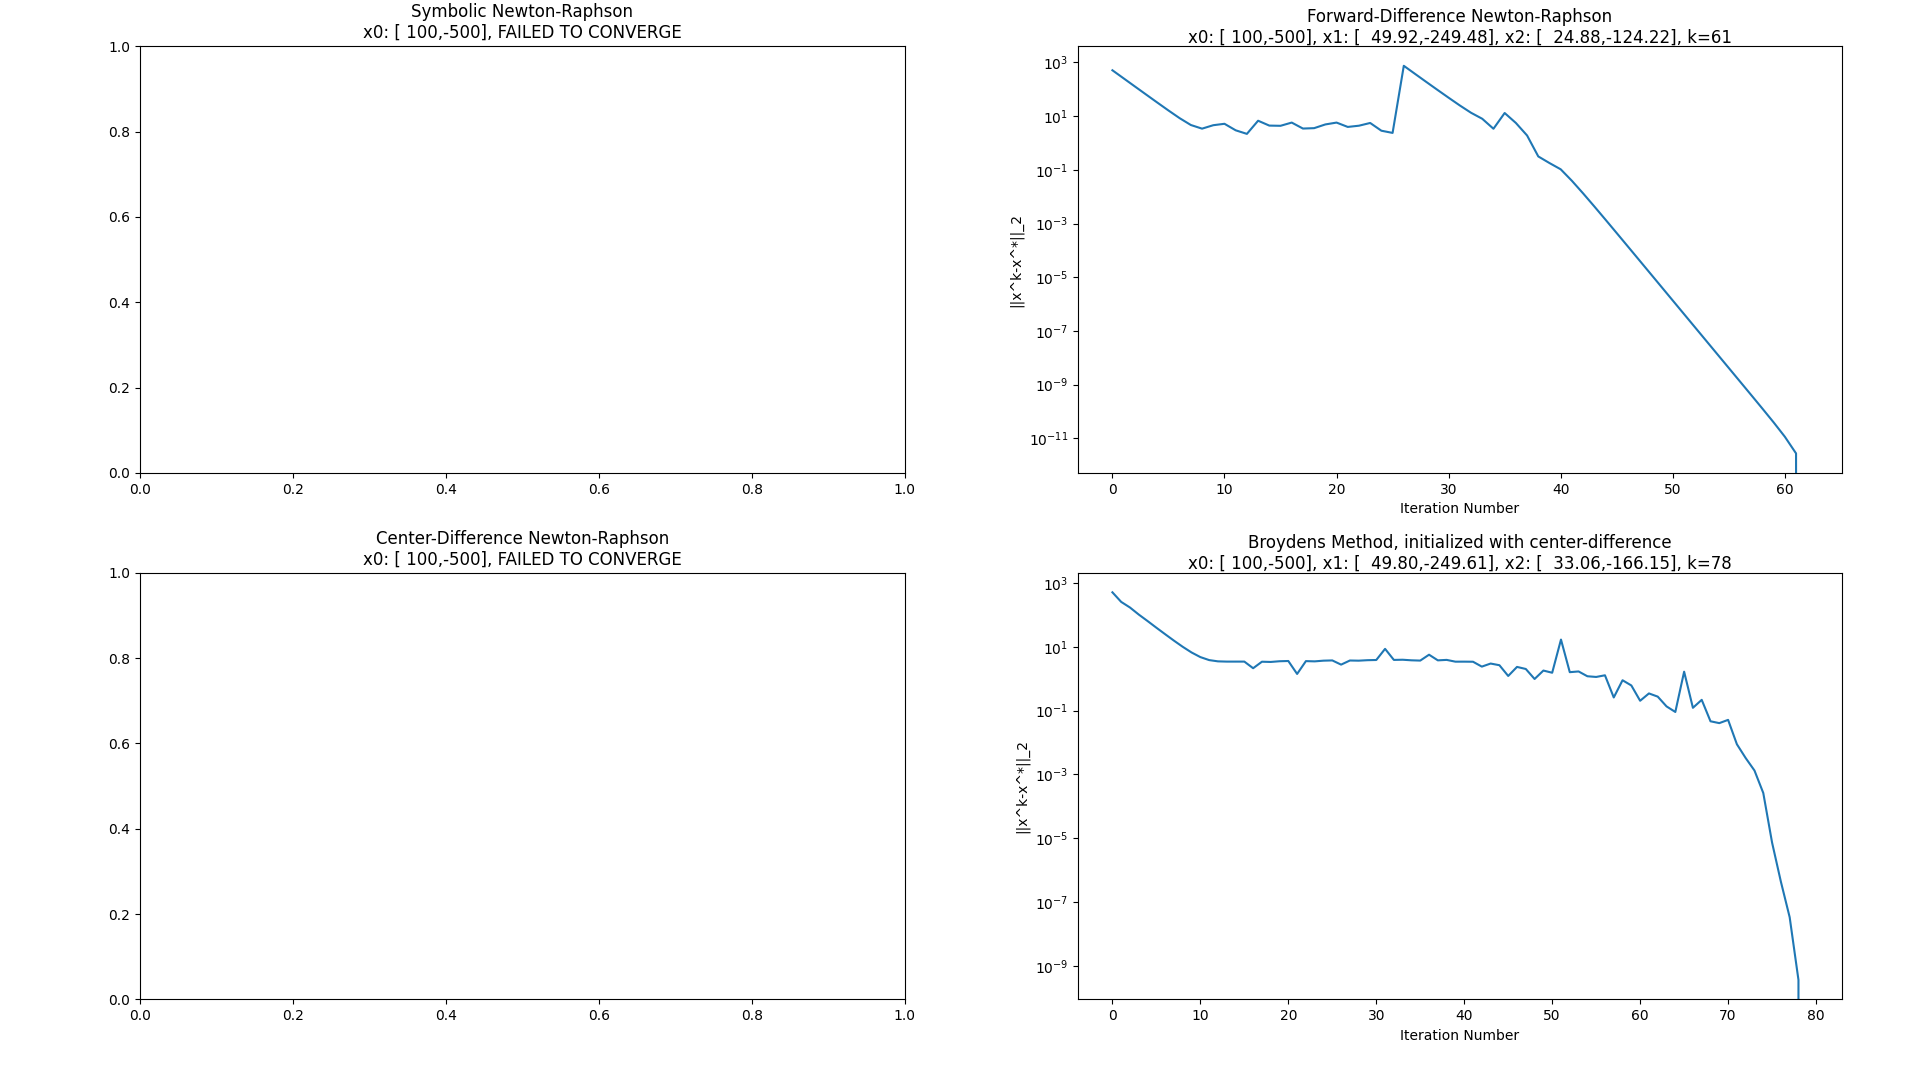
\includegraphics[width=1.25\textwidth, angle=90]{Figure_4.png}
	\caption{The four methods, started from $(100, -500)$}
\end{figure}

%--------------------------------------

\newpage
\section*{Problem 2: Understanding Numerical Differentiation}
\subsection*{Problem Statement}
We have empirically seen in class that the approximation quality of center
difference approximation is far superior to that of forward and backward
difference ones, when performing numerical differentiation. In this problem, we
gain analytical insight into this behavior.

Suppose $f : \mathbb{R}\rightarrow\mathbb{R}$ is at least $C^3$ over $[a,b]$. The following
Taylor's series expansion of $f$ might be useful:
\[
	f(x+h) = f(x) + hf'(x) + \frac{h^2}{2}f''(x)+\frac{h^3}{6}f'''(\zeta)
\]
$\forall x, x+h\in(a,b)$ where $\zeta$ lies on the line segment joining $x$ and $x+h$.

\subsubsection*{a}
Show that
\[
	\left|
	\frac{f(x+h)-f(x)}{h}-f'(x)
	\right|
	\leq M|h|
	\forall x\in(a,b), M>0
\]

\subsubsection*{b}
Show that
\[
	\left|
	\frac{f(x+h)-f(x-h)}{2h}-f'(x)
	\right|
	\leq N|h|^2
	\forall x\in(a,b), N>0
\]
\subsubsection*{c}
Qualitatively discuss what the results in (a) and (b) mean.

\subsection*{Solution}
\subsubsection*{a}
Re-arrange the provided Taylor series expansion and take the absolute value of both sides:
\[
	\left|\frac{f(x+h)-f(x)}{h} - f'(x)\right|
	= \left|h(\frac{1}{2}f''(x)+\frac{1}{6}hf'''(\zeta))\right|
	= \left|h\right|\left|\frac{1}{2}f''(x)+\frac{1}{6}hf'''(\zeta)\right|
\]
Now we just need to bound the rightmost absolute value. From the class notes
(``Solving nonlinear equations''), note that because $\zeta$ lies on the line
segment connecting $a$ and $b$, $\zeta\in[a,b]$. Because the function is $C^3$
over $[a,b]$, there exists a scalar $M_1$ and $M_2$ that bounds $f''$ and $f'''$
(repsectively) from above. So:
\[
	\left|\frac{1}{2}f''(x)+\frac{1}{6}hf'''(\zeta)\right|
	\leq\left|\frac{1}{2}M_1 + \frac{1}{6}hM_2\right|
\]
Finally, because $h$ is some fixed value, the whole quantity is bounded, and we can say:
\[
	\left|\frac{1}{2}M_1 + \frac{1}{6}hM_2\right|
	\leq M
\]
\[
	\therefore
	\left|\frac{f(x+h)-f(x)}{h} - f'(x)\right|
	\leq M|h|
\]
\qed
\subsubsection*{b}
We can modify the expansion to consider a negative $h$, or equivalently the subtraction of
a positive $h$:
\[
	f(x-h) = f(x) - hf'(x) + \frac{h^2}{2}f''(x)-\frac{h^3}{6}f'''(\zeta)
\]
Then, subtract the two series to find:
\[
	f(x+h)-f(x-h)
	= f(x)+hf'(x)+\frac{h^2}{2}f''(x)+\frac{h^3}{6}f'''(\zeta)
	- f(x)+hf'(x)-\frac{h^2}{2}f''(x)+\frac{h^3}{6}f'''(\zeta)
\]
\[
	= 2hf'(x)+\frac{2h^3}{6}f'''(\zeta)
\]
Rearranging:
\[
	\frac{f(x+h)-f(x-h)}{2h} -f'(x)
	= \frac{h^2}{6}f'''(\zeta)
\]
\[
	\left|\frac{f(x+h)-f(x-h)}{2h} -f'(x)\right|
	= \left|\frac{h^2}{6}f'''(\zeta)\right|
	= \left|h^2\right|\left|\frac{1}{6}f'''(\zeta)\right|
\]
By the same logic as in (2.a), we know that $f'''(\zeta)$ is upper bounded, so we can say:
\[\frac{1}{6}f'''(\zeta)\leq N\]
Thus:
\[
	\left|\frac{f(x+h)-f(x-h)}{2h} -f'(x)\right|
	\leq \left|h^2\right|N
\]
\qed

\subsubsection*{c}
As the proofs show, there's a cancellation effect that occurs for some of the more significant
error terms, resulting in the far better approximation (at least for ``small'' $h$).
There's an ``averaging'' effect that reduces the error.

Expanding on the numerical example provided in class, it's worth
looking at it as a form of a statistical filter\footnote{Note: I'm not
	exactly a wizard at stats, take this with a grain of salt...}. Some
``signal'' (the error of the approximation) is oversampled at a $2x$ rate and then is
passed through an averaging filter. Assume that:
\begin{enumerate}
	\item The samples are uncorrelated
	\item The distribution of each sample is \textit{normal}
\end{enumerate}
which seems justified based on the numerical results presented in class.
Then, letting $X_i$ denote the distribution of the samples (where $i=1,2$), and
$\overline{X}$ denote the average (i.e. the output of the filter), we can say:
\[
	\mathrm{Var}(\overline{X})
	= \mathrm{Var}\left(\frac{1}{N}\sum_{i=1}^N X_i\right)
	= \mathrm{Var}\left(\frac{1}{N}\sum_{i=1}^N X_i\right)
	= \frac{1}{N^2}\mathrm{Var}\left(\sum_{i=1}^N X_i\right)
	= \frac{1}{N^2}\sum_{i=1}^N \mathrm{Var}\left(X_i\right)
\]
If the variances are the same ($X_1 = X_2 = X$), then we get:
\[ \mathrm{Var}(\overline{X}) = \frac{1}{2}\mathrm{Var}(X) \]
Now, this doesn't seem to imply quite aggressive reduction in variance as demonstrated by the numerical example
given in class, but it's at least a way to start thinking about how this works.

\newpage
\section*{Code Listing}
\definecolor{codegreen}{rgb}{0,0.6,0}
\definecolor{codegray}{rgb}{0.5,0.5,0.5}
\definecolor{codepurple}{rgb}{0.58,0,0.82}
\definecolor{backcolour}{rgb}{0.95,0.95,0.92}
\lstdefinestyle{mystyle}{
	backgroundcolor=\color{backcolour},
	commentstyle=\color{codegreen},
	keywordstyle=\color{magenta},
	numberstyle=\tiny\color{codegray},
	stringstyle=\color{codepurple},
	basicstyle=\ttfamily\footnotesize,
	breakatwhitespace=false,
	breaklines=true,
	captionpos=b,
	keepspaces=true,
	numbers=left,
	numbersep=5pt,
	showspaces=false,
	showstringspaces=false,
	showtabs=false,
	tabsize=2
}
\lstset{style=mystyle}
\lstinputlisting[
	language=Python,
	basicstyle=\tiny
]{../../ece530/ece530/hw1/__main__.py}

\end{document}
